% !TeX root = ../main.tex

\section{Introduzione}
In questo capitolo vengono mostrati i risultati ottenuti dalla realizzazione della applicazione multipiattaforma MaggioliEbook adottando il processo di sviluppo descritto nel capitolo \ref{ch:cicd}.

Vengono inizialmente considerati i requisiti definiti nel capitolo \ref{ch:casodistudio} e paragonati con quanto realizzato. Successivamente sono indicate alcune statistiche e metriche, raccolte principalmente tramite la piattaforma GitLab adottata, al fine di creare un primo modello di confronto per i lavori futuri che saranno svolti in azienda sulle tematiche principali di questo caso di studio industriale.

\section{Riuso}
I template che definiscono gli stage e i relativi job del processo di sviluppo progettato sono stati versionati e organizzati in un apposito repository, come descritto in modo dettagliato nel capitolo \ref{ch:cicd}.

Questa soluzione non solo permette il riuso dell'intera pipeline o di solamente una sua parte, ma abilita anche un processo di lavoro collaborativo fra tutti i possibili utilizzatori per la modifica del processo. Ogni sviluppatore all'interno della azienda è infatti in grado di accedere al repository dei template, visionare i file YAML che definiscono la pipeline e aprire merge request per richiedere la modifica o l'aggiunta di funzionalità necessarie al processo di sviluppo automatizzato. A tal proposito è stato scelto un team di sviluppo all'interno dell'azienda che si occupa di applicazioni mobile per svolgere un primo esperimento di integrazione nel proprio processo di sviluppo, già consolidato su tecnologie puramente native e senza alcun sistema di automazione.

\section{Stabilizzazione e rilascio}
La fase di stabilizzazione e rilascio di entrambe le versioni di applicazione sviluppate tramite Kotlin Multiplatform Mobile sono state realizzate rispettando tutti i vincoli definiti nel capitolo \ref{ch:casodistudio}. Durante il processo di sviluppo del caso di studio è stato infatti possibile rilasciare automaticamente applicazioni, sia Android che iOS, sfruttando la pipeline realizzata. In entrambi i casi sono stati definiti gruppi di tester composti sia dalle figure aziendali esperte di dominio che dai Professori relatori di questa tesi:

\begin{figure}[H]
    \centering
    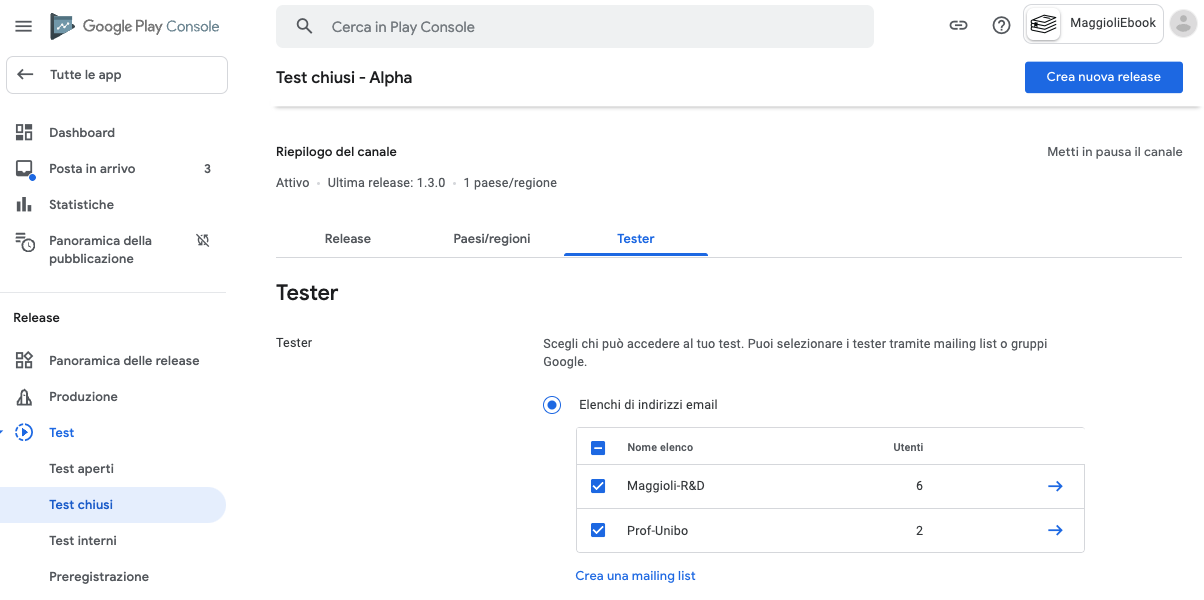
\includegraphics[width=1\textwidth]{img/google-play-console-maggioliebook.png}
    \caption{Schermata Google Play Console per la fase di stabilizzazione della applicazione Android}
    \label{google-play-console-maggioliebook}
\end{figure}

\begin{figure}[H]
    \centering
    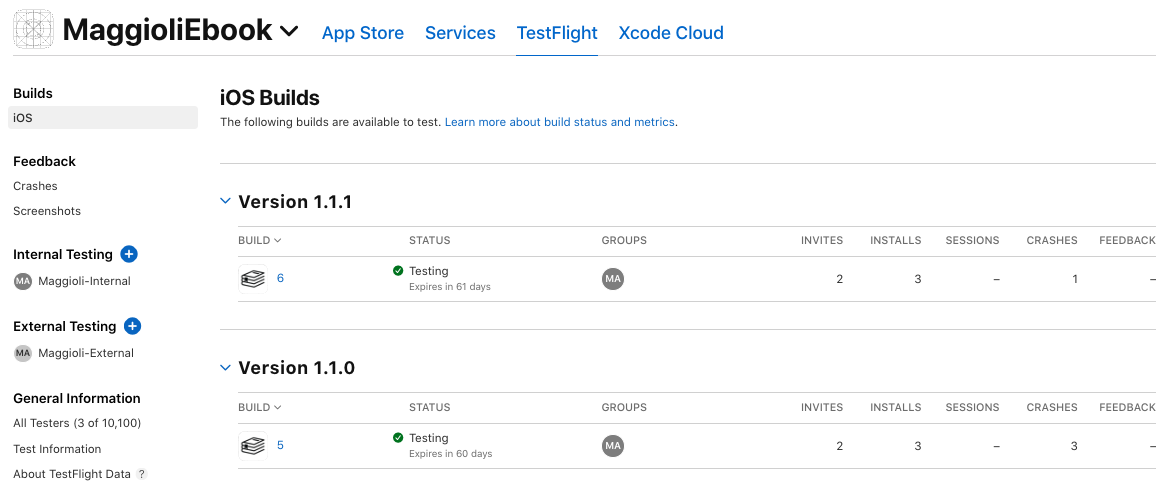
\includegraphics[width=1\textwidth]{img/app-store-connect-maggioliebook.png}
    \caption{Schermata App Store Connect per la fase di stabilizzazione della applicazione iOS}
    \label{app-store-connect-maggioliebook}
\end{figure}

Tutti i tester appartenenti ai gruppi configurati come nelle schermate precedenti sono poi stati in grado di installare con successo l'applicazione sul proprio dispositivo:

\begin{figure}[H]
    \centering
    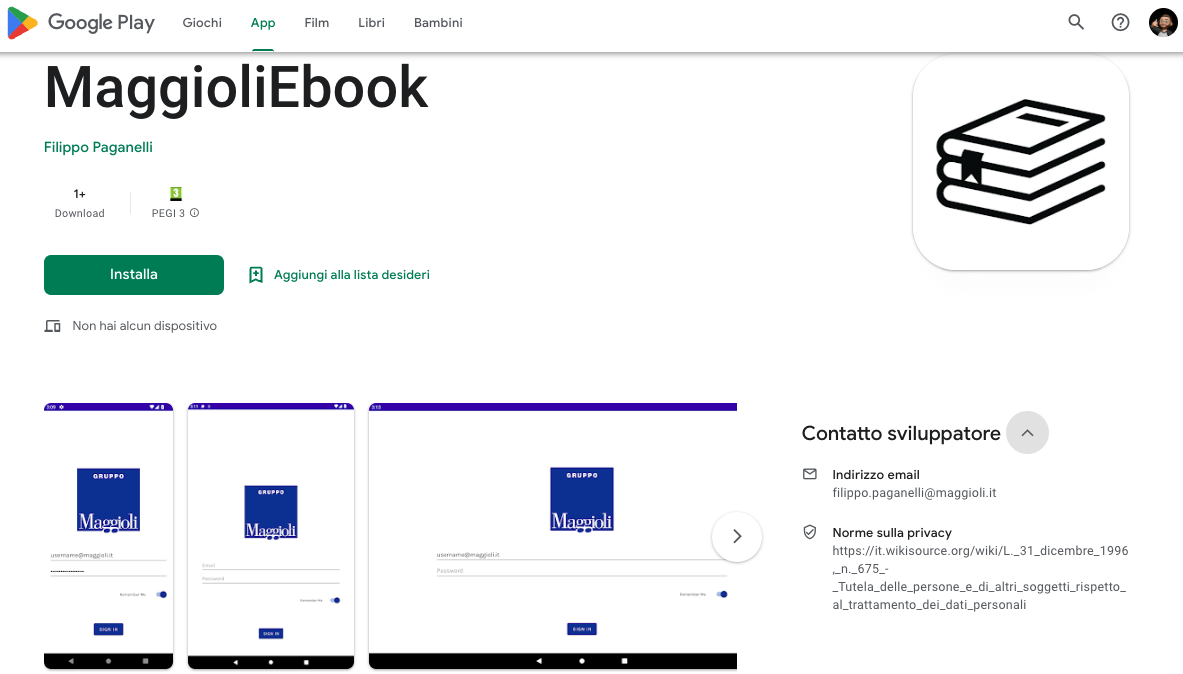
\includegraphics[width=1\textwidth]{img/google-play-store-maggioliebook.png}
    \caption{Schermata Google Play Store per la fase di stabilizzazione della applicazione Android}
    \label{google-play-store-maggioliebook}
\end{figure}

\begin{figure}[H]
    \centering
    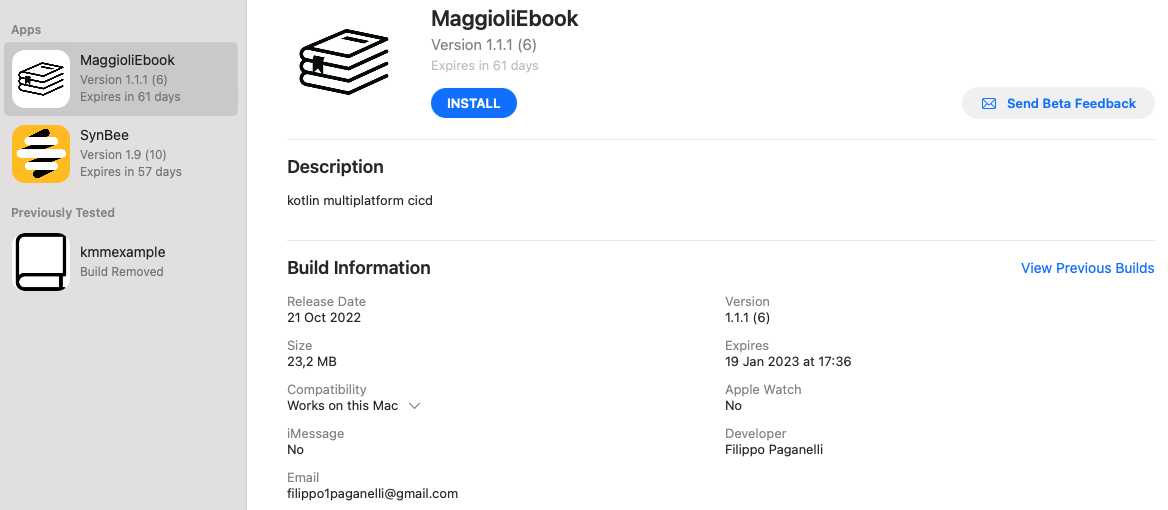
\includegraphics[width=1\textwidth]{img/testflight-maggioliebook.png}
    \caption{Schermata Testflight per la fase di stabilizzazione della applicazione iOS}
    \label{testflight-maggioliebook}
\end{figure}

Un ciclo di stabilizzazione \textit{alpha}-\textit{beta} risulta nell'esecuzione di due pipeline attivate rispettivamente con (\textit{i}) la modifica sul branch \textit{dev} del codice della applicazione e (\textit{ii}) il merge del branch \textit{dev} sul branch \textit{test}. Le seguenti schermate, catturate dalla piattaforma GitLab utilizzata come sistema di versionamento e automazione, mostrano l'esecuzione di un esempio di queste due pipeline nel caso della sola applicazione Android:

\begin{figure}[H]
\centering
    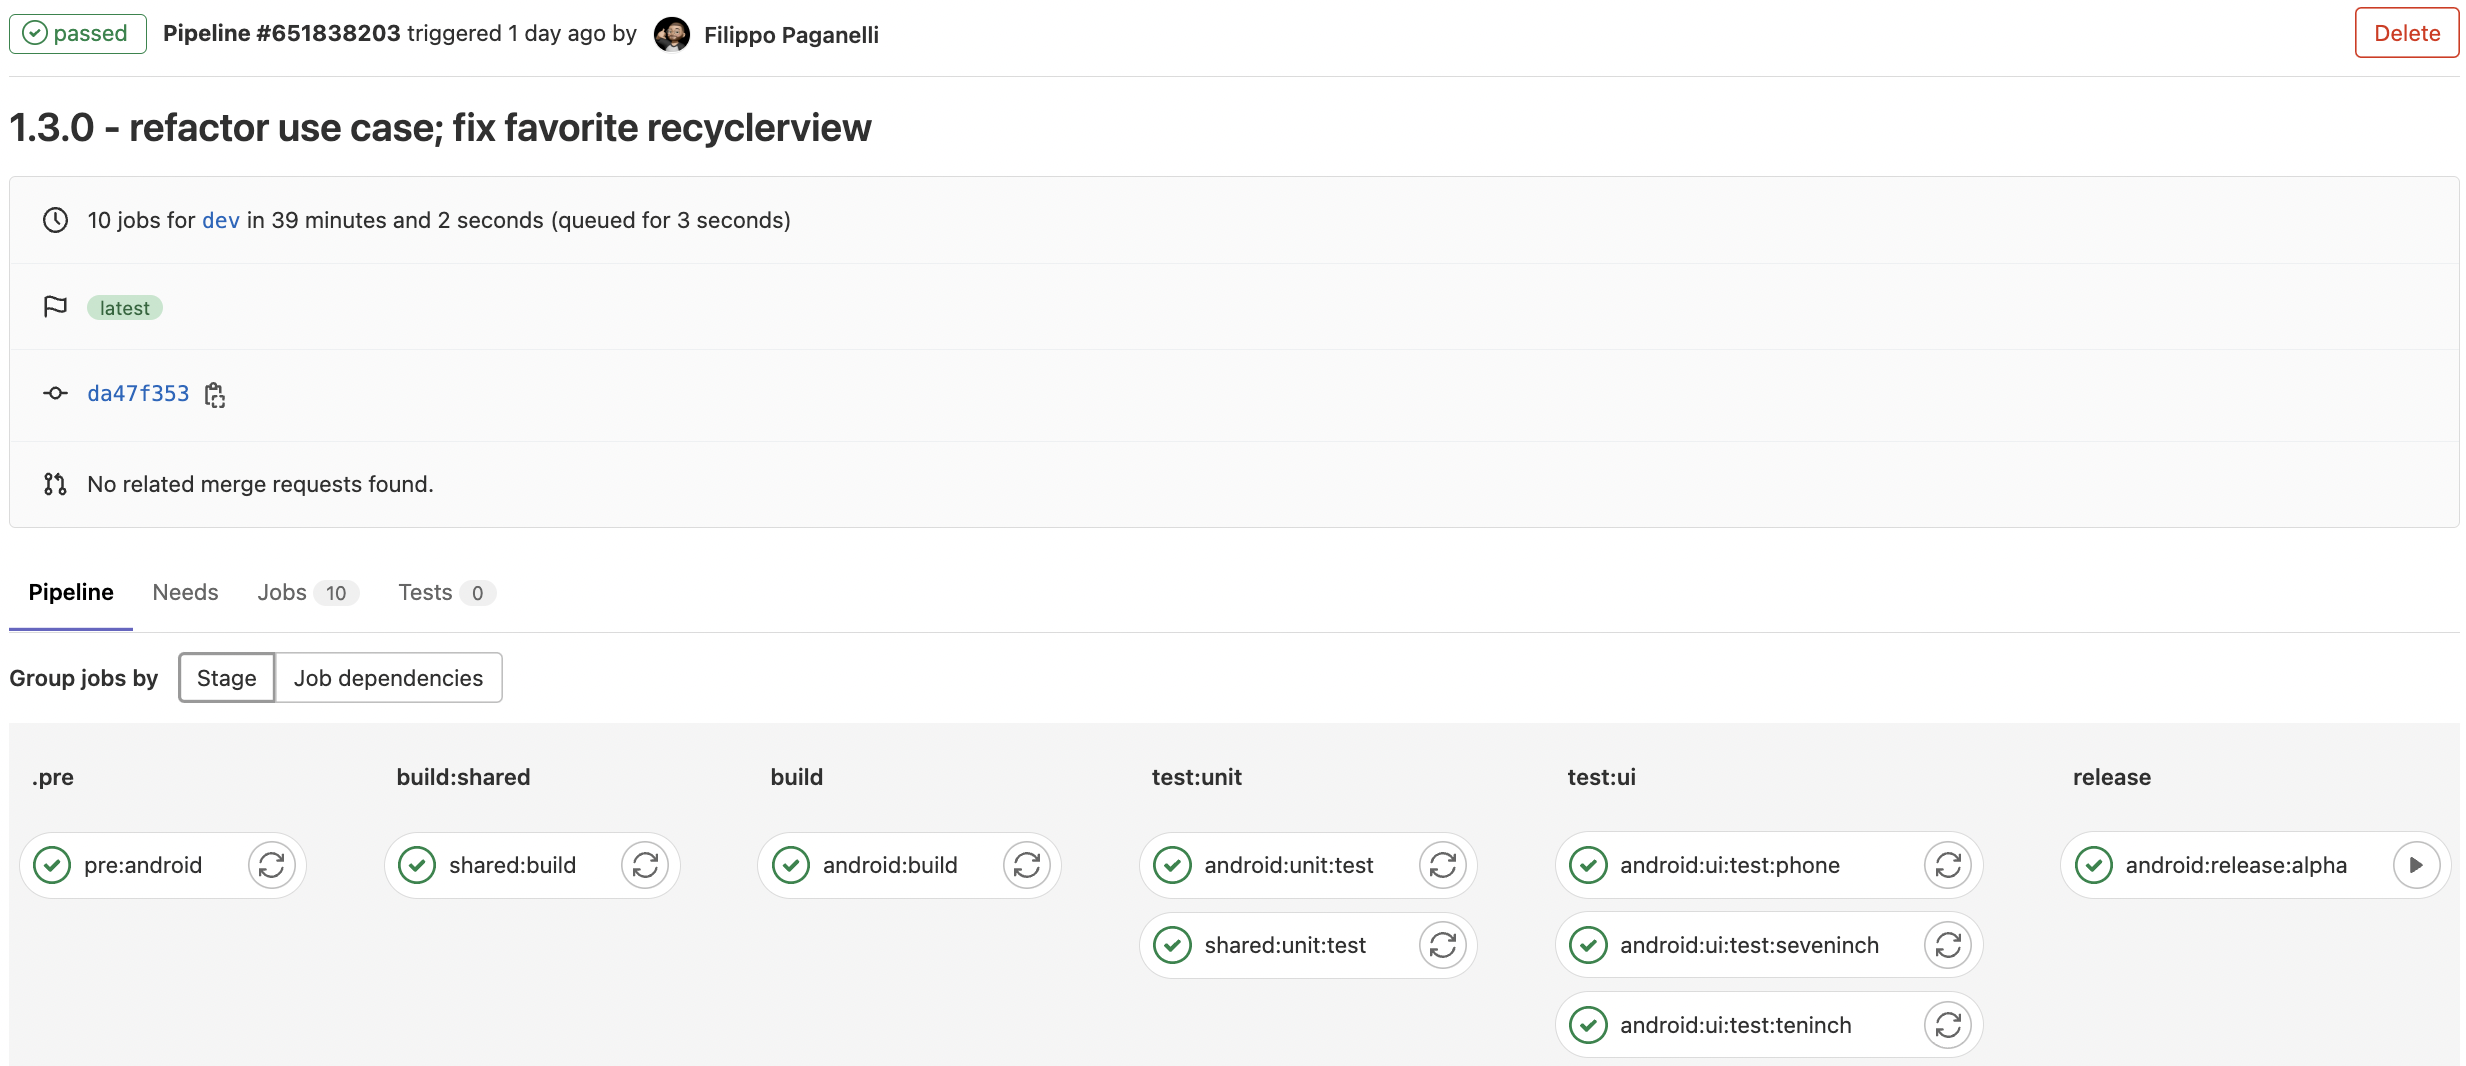
\includegraphics[width=1\textwidth]{img/gitlab-pipeline-android-alpha.png}
    \caption{Schermata GitLab di esecuzione della pipeline completa per il rilascio della applicazione Android in versione \textit{alpha}}
    \label{gitlab-pipeline-android-alpha}
\end{figure}

\begin{figure}[H]
\centering
    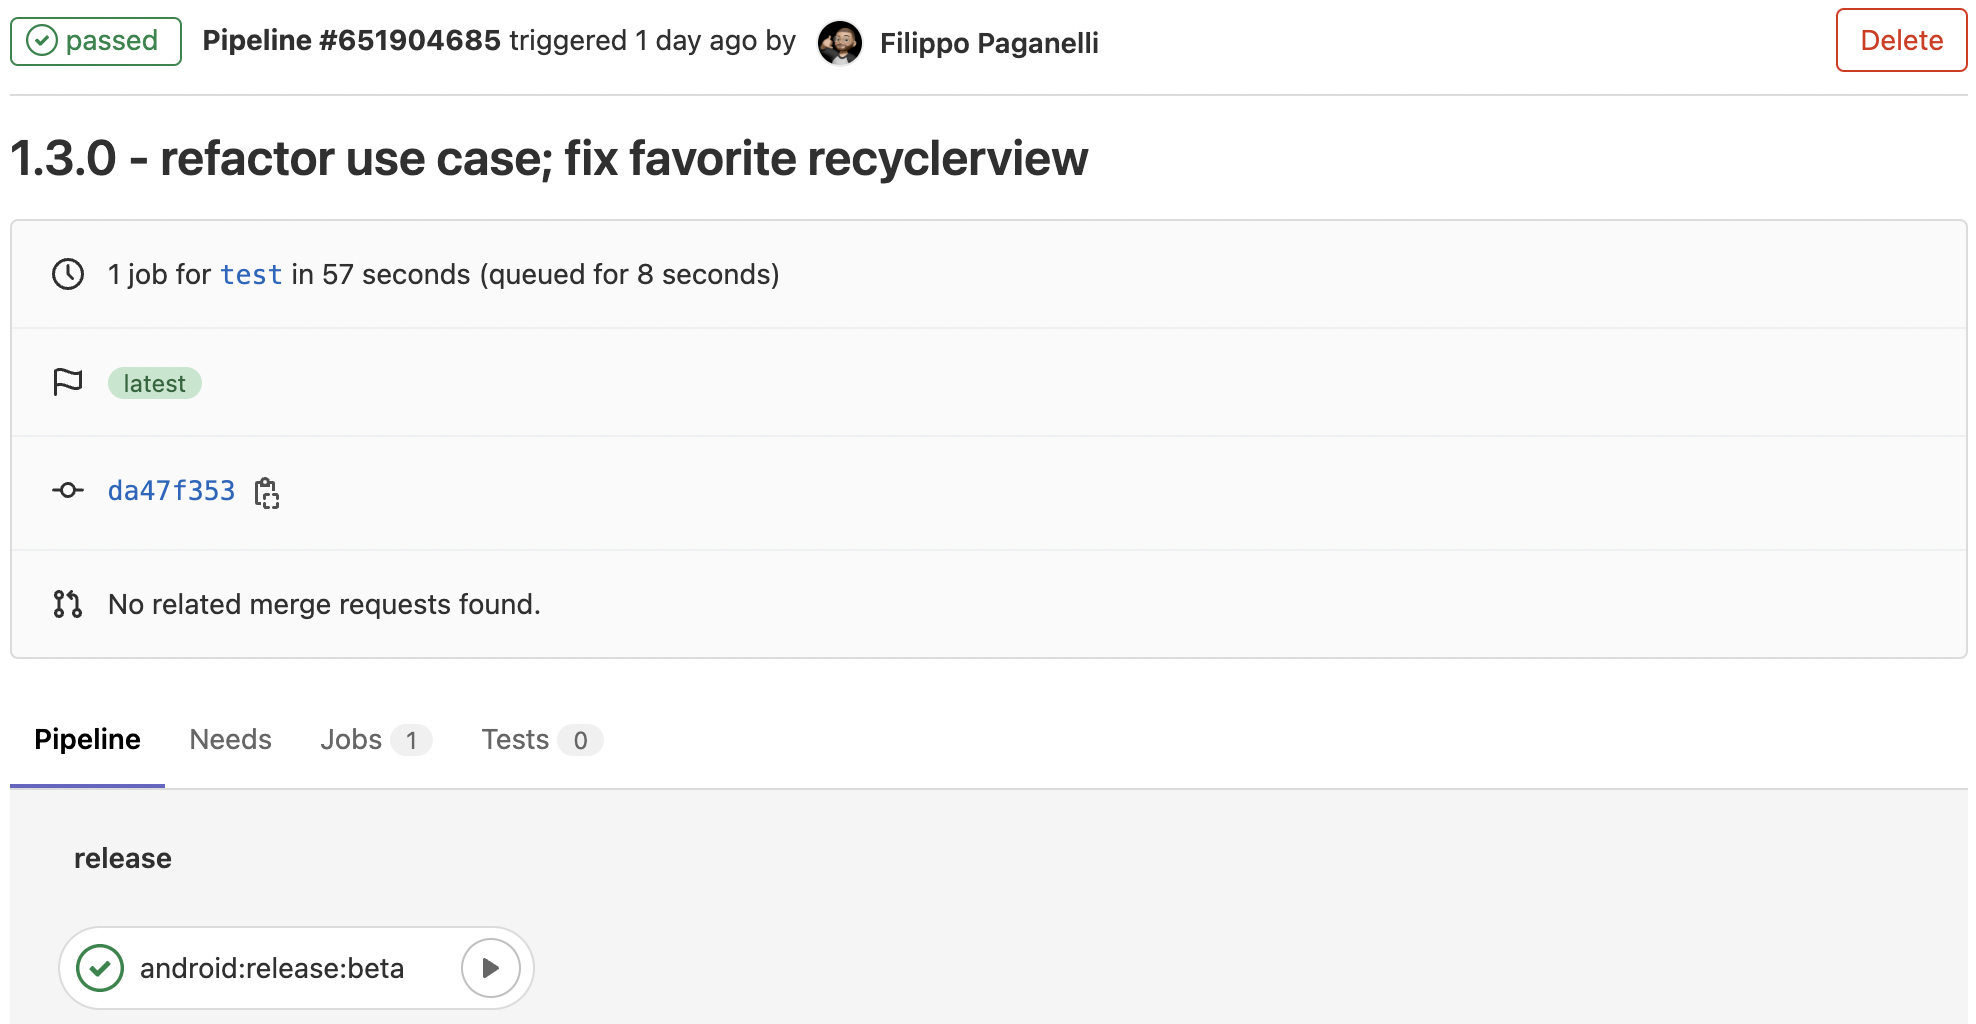
\includegraphics[width=1\textwidth]{img/gitlab-pipeline-android-beta.png}
    \caption{Schermata GitLab di esecuzione della pipeline completa per la promozione da versione \textit{alpha} a versione \textit{beta} della applicazione Android}
    \label{gitlab-pipeline-android-beta}
\end{figure}

\section{Analisi del codice}
% efficacia della pipeline di analisi

\section{Statistiche}
% qualche misurazione delle tempistiche di esecuzione delle pipeline nei vari casi (android, ios, ios+android e rilascio, analisi, ...)
% non ho parametri per fare il confronto rispetto a prima, la app sviluppata è nuova e altri team non hanno cicd app mobile

\section{Lavori futuri}
% cosa ho intenzione di fare dopo, continuazione del lavoro in azienda
\begin{itemize}
        \item Studio, ricerca e sperimentazione per la fase di monitoring, sia della applicazione che dell'utente.
        \item Utilizzo del meccanismo \textit{Remote Configuration}\footnote{\url{https://firebase.google.com/docs/remote-config}} per modificare aspetti della applicazione in modo dinamico senza dover rilasciare nuove versioni. Un esempio tipico è la migrazione dei database: grazie al meccanismo di remote configuration è possibile settare da remoto il \textit{jdbc}\footnote{Java DataBase Connectivity} url che permette di connettersi al database senza dover rilasciare una nuova versione della applicazione con il valore cablato nel codice.
        \item Valutazione di alternative all'hardware Apple fisico. Come indicato nel capitolo \ref{ch:cicd} alcune possibilità individuate sono: (\textit{i}) runner gestiti con sistema operativo MacOS (disponibili su diverse piattaforme come GitLab\footnote{\url{https://docs.gitlab.com/ee/ci/runners/saas/macos_saas_runner.html}}, GitHub\footnote{\url{https://docs.github.com/en/actions/using-github-hosted-runners/about-github-hosted-runners}} e CircleCI\footnote{\url{https://circleci.com/docs/using-macos}}), (\textit{ii}) virtual machine as-a-Service con sistema operativo MacOS (disponibili tra i servizi cloud Amazon\footnote{\url{https://aws.amazon.com/ec2/instance-types/mac/}}) e (\textit{iii}) immagine Docker MacOS\footnote{\url{https://github.com/sickcodes/Docker-OSX}}.
        \item Separazione dei moduli sviluppati in questo caso di studio in modo da avere più repository separati invece che la soluzione monorepo adottata. Distribuzione della logica applicativa sotto forma di libreria kmm e valutazione dei pro e contro di questa soluzione.
        \item Valutazione soluzioni complete as-a-Service. Ad esempio \textit{Bitrise}\footnote{\url{https://www.bitrise.io/}} o XCode Cloud\footnote{\url{https://developer.apple.com/documentation/xcode/xcode-cloud}} (solamente per la parte Apple).
        \item Sperimentazione tecniche CI/CD con tecnologie cross-platform come \textit{Ionic}\footnote{\url{https://ionicframework.com/}}, \textit{Flutter}\footnote{\url{https://flutter.dev/}} o \textit{React Native}\footnote{\url{https://reactnative.dev/}} e stesso caso d'uso (applicazione PoC MaggioliEbook) in modo da avere dei parametri di riferimento e confronto.
\end{itemize}